\chapter{The knee and its twelve findings}
\label{ch:knee}

\begin{tldr}
\begin{itemize}
\item The knee is where the thigh bone (femur) meets the shin bone (tibia); the kneecap (patella) glides in front.
\item Four kinds of parts can go wrong: \textbf{ropes} (ligaments), \textbf{cushions} (menisci),
      \textbf{surfaces} (cartilage), and \textbf{fluid and bone}.
\item The 12 findings are those parts, split into \textbf{medial} (inner) and \textbf{lateral} (outer) where it matters.
\item ``Positive'' means \textbf{severe enough}: a small effusion or a mild sprain counts as \emph{negative}.
\end{itemize}
\end{tldr}

\section{The parts of a knee}

\begin{wordcheck}
\term{Medial} = towards the middle of the body (the inner side of the knee). \term{Lateral} = away from the
middle (the outer side). \term{Anterior} = front, \term{posterior} = back. These words name the findings:
\emph{medial} meniscus, \emph{lateral} OA, \emph{anterior} cruciate ligament.
\end{wordcheck}

\paragraph{The parts in one line each.}
\begin{itemize}
\item \textbf{Bones:} femur on top, tibia below, patella in front, fibula on the outer side of the tibia.
\item \textbf{Cartilage:} a smooth layer (2--4\,mm) on the bone ends, so they glide.
\item \textbf{Menisci:} two C-shaped rubbery cushions between femur and tibia, one medial, one lateral.
\item \textbf{Ligaments:} ropes that hold the bones together. The two \textbf{cruciates} (ACL, PCL) cross inside
      the knee; the two \textbf{collaterals} (MCL inner, LCL outer) run along the sides.
\item \textbf{Synovium and joint fluid:} the joint is a sealed bag lined by the synovium, with a little lubricating
      fluid inside. The bag has a big pocket above the kneecap where extra fluid collects.
\end{itemize}

\begin{figure}[H]
\centering
\begin{tikzpicture}[scale=0.5]
  \kneesagittal
  \klabel{(3.05,10.9)}{(-0.4,11.0)}{east}{Quadriceps tendon}
  \klabel{(3.78,9.4)}{(-0.4,9.4)}{east}{Joint fluid\\(top pocket)}
  \klabel{(2.85,7.55)}{(-0.4,7.7)}{east}{Patella\\(kneecap)}
  \klabel{(3.42,6.2)}{(-0.4,6.1)}{east}{Cartilage}
  \klabel{(3.3,5.0)}{(-0.4,4.75)}{east}{Patellar tendon}
  \klabel{(4.0,4.75)}{(-0.4,3.3)}{east}{Meniscus\\(front horn)}
  \klabel{(5.5,10.4)}{(10.8,10.6)}{west}{Femur\\(thigh bone)}
  \klabel{(8.05,6.3)}{(10.8,7.9)}{west}{Back of the knee\\(Baker's cyst site)}
  \klabel{(5.45,5.55)}{(10.8,6.15)}{west}{ACL}
  \klabel{(6.95,5.4)}{(10.8,4.95)}{west}{PCL}
  \klabel{(7.05,4.8)}{(10.8,3.75)}{west}{Meniscus\\(back horn)}
  \klabel{(5.45,1.8)}{(10.8,1.8)}{west}{Tibia\\(shin bone)}
  \node[font=\scriptsize\sffamily\bfseries, text=muted] at (1.0,-0.8) {FRONT};
  \node[font=\scriptsize\sffamily\bfseries, text=muted] at (9.2,-0.8) {BACK};
\end{tikzpicture}\hspace{4mm}
\begin{tikzpicture}[scale=0.5]
  \kneecoronal
  \klabel{(2.2,6.0)}{(-0.4,7.9)}{east}{LCL}
  \klabel{(3.3,4.87)}{(-0.4,6.2)}{east}{Cartilage}
  \klabel{(2.7,4.8)}{(-0.4,4.6)}{east}{Lateral\\meniscus}
  \klabel{(2.15,1.6)}{(-0.4,1.9)}{east}{Fibula}
  \klabel{(5.0,10.2)}{(10.4,10.6)}{west}{Femur}
  \klabel{(5.02,5.2)}{(10.4,8.7)}{west}{ACL + PCL\\(in the notch)}
  \klabel{(7.84,5.7)}{(10.4,6.5)}{west}{MCL}
  \klabel{(7.3,4.8)}{(10.4,4.6)}{west}{Medial\\meniscus}
  \klabel{(5.0,1.8)}{(10.4,1.9)}{west}{Tibia}
  \node[font=\scriptsize\sffamily\bfseries, text=muted] at (2.2,-0.8) {LATERAL};
  \node[font=\scriptsize\sffamily\bfseries, text=muted] at (7.8,-0.8) {MEDIAL};
\end{tikzpicture}
\caption{Left: a knee seen from the side (front of the leg on the left, as in the MRI images later). Right: a
right knee seen from the front. Blue wedges = menisci, light blue = cartilage, red = ligaments.}
\label{fig:anatomy}
\end{figure}

\section{Three compartments}

Doctors split the knee into three areas where two cartilage surfaces touch. Three of our findings are
``osteoarthritis in compartment X''.

\begin{figure}[H]
\centering
\begin{tikzpicture}[scale=0.42]
  \kneecoronal
  \fill[them, opacity=0.28, rounded corners=3pt] (1.9,4.0) rectangle (4.75,5.6);
  \fill[us, opacity=0.28, rounded corners=3pt] (5.25,4.0) rectangle (8.1,5.6);
  \node[font=\scriptsize\sffamily\bfseries, text=them!80!black, align=center] at (2.6,-0.9) {lateral\\[-1pt]compartment};
  \node[font=\scriptsize\sffamily\bfseries, text=us!80!black, align=center] at (7.4,-0.9) {medial\\[-1pt]compartment};
\end{tikzpicture}\hspace{10mm}
\begin{tikzpicture}[scale=0.42]
  \kneesagittal
  \fill[third, opacity=0.35, rotate around={-8:(2.85,7.55)}, rounded corners=3pt] (2.95,6.2) rectangle (3.9,8.9);
  \node[font=\scriptsize\sffamily\bfseries, text=third!70!black, align=center] at (2.4,-0.9) {patellofemoral\\[-1pt]compartment};
\end{tikzpicture}
\caption{\textbf{Medial OA} and \textbf{Lateral OA} are about the two tibiofemoral compartments (femur on tibia,
left). \textbf{PF OA} is about the patellofemoral compartment, where the kneecap glides on the femur (right).}
\label{fig:compartments}
\end{figure}

\section{The twelve findings, one card each}

Every card says what the finding is, when it counts as \textbf{positive} in this competition, and where it is
easiest to see (the planes are explained in Chapter~\ref{ch:mri}).

\newcommand{\findingcard}[5]{%
  \begin{tcolorbox}[enhanced, colback=white, colframe=grid, boxrule=0.5pt, arc=1.2mm,
     title={#1}, fonttitle=\bfseries\small, coltitle=ink, colbacktitle=keyfill,
     left=2mm, right=2mm, top=1mm, bottom=1mm, fontupper=\footnotesize]
  #2\par\smallskip
  \textcolor{wordline}{\faCheckCircle}\ \textbf{Positive if:} #3\par
  \textcolor{muted}{\faTimesCircle}\ \textbf{Negative:} #4\par
  \textcolor{accent}{\faEye}\ \textbf{Best seen:} #5
  \end{tcolorbox}}

\begin{tcbraster}[raster columns=2, raster equal height=rows, raster column skip=3mm, raster row skip=2.5mm]
\findingcard{ACL (anterior cruciate ligament)}
  {The rope in the middle of the knee that stops the shin bone sliding forward. Torn by twisting, typical in football and skiing.}
  {high-grade partial or complete tear (more than half the fibres).}
  {sprain, low-grade partial tear, signal change only.}
  {sagittal images.}
\findingcard{MCL (medial collateral ligament)}
  {The rope on the inner side. Torn when the knee is hit from the outside.}
  {acute high-grade or complete tear.}
  {low-grade sprain, old scarring.}
  {coronal images.}
\findingcard{Medial meniscus}
  {The inner cushion. Tears from twisting, or from wear in older knees.}
  {a tear reaching the meniscus surface (seen on $\geq$2 images), or a deformed meniscus.}
  {degeneration inside the meniscus that does not reach the surface.}
  {sagittal and coronal.}
\findingcard{Lateral meniscus}
  {The outer cushion. Same as the medial one, on the other side.}
  {same rule as the medial meniscus.}
  {same rule.}
  {sagittal and coronal.}
\findingcard{Medial OA (osteoarthritis)}
  {Cartilage worn away between femur and tibia on the inner side. The most common place for knee arthritis.}
  {an area of about 1\,cm or more where more than half of the cartilage thickness is lost.}
  {softening, thin fissures, small defects.}
  {coronal and sagittal.}
\findingcard{Lateral OA}
  {The same wear on the outer side.}
  {same rule, lateral compartment.}
  {same rule.}
  {coronal and sagittal.}
\findingcard{PF OA (patellofemoral)}
  {Cartilage worn between the kneecap and the groove of the femur.}
  {same rule, patellofemoral compartment.}
  {same rule.}
  {axial and sagittal.}
\findingcard{Effusion}
  {Too much fluid in the joint bag. A sign that something inside is irritated or injured.}
  {moderate or large amount.}
  {trace, small or ``physiological'' fluid.}
  {sagittal (pocket above the kneecap) and axial.}
\findingcard{Synovitis}
  {The lining of the joint is thickened and inflamed. Hard to see without contrast dye; reports often do not mention it.}
  {thickened, inflamed synovium.}
  {normal lining; fluid alone is not synovitis.}
  {axial and sagittal.}
\findingcard{Baker's cyst}
  {A fluid sac behind the knee, a bulge of the joint bag between two muscles.}
  {moderate or large cyst.}
  {small or tiny cyst.}
  {axial and sagittal.}
\findingcard{Contusion (bone bruise)}
  {Bleeding and swelling inside the bone after an impact. Bright on fat-suppressed images. Classic companion of an ACL tear.}
  {impact bone-marrow edema without a fracture line.}
  {edema from wear or overload.}
  {fat-suppressed fluid-sensitive images, any plane.}
\findingcard{Fracture}
  {A broken bone.}
  {an acute fracture line or break in the outer bone layer (cortex).}
  {old healed fractures.}
  {a line on T1 or PD images, with edema around it on fat-suppressed images.}
\end{tcbraster}

\section{``Positive'' means ``past a threshold''}

The doctors who made the reference labels used strict rules: a finding only counts if it is severe enough,
and a borderline case counts as \textbf{negative}. This matters a lot, because a radiology report mentions
small things too (``small effusion'', ``grade 1 sprain'').

\begin{figure}[H]
\centering
\begin{tikzpicture}[x=0.86mm,y=1mm]
  \foreach \y/\name/\neg/\pos in {0/Effusion/{none \quad trace \quad small}/{moderate \quad large},
                                 -11/ACL/{intact \quad sprain \quad low-grade tear}/{high-grade tear \quad complete},
                                 -22/Cartilage (OA)/{normal \quad softening \quad $<$50\,\% loss}/{$>$50\,\% loss over \ca 1\,cm}} {
    \node[anchor=east, font=\footnotesize\bfseries] at (-2,\y) {\name};
    \fill[grid] (0,\y-3) rectangle (78,\y+3);
    \fill[them!70] (78,\y-3) rectangle (140,\y+3);
    \node[font=\scriptsize] at (39,\y) {\neg};
    \node[font=\scriptsize, text=white] at (109,\y) {\textbf{\pos}};
  }
  \draw[ink, line width=1pt, dashed] (78,6) -- (78,-28);
  \node[font=\scriptsize\bfseries, anchor=south] at (78,6) {threshold};
  \node[font=\scriptsize, text=muted] at (39,9) {label = 0 (negative)};
  \node[font=\scriptsize, text=them!80!black] at (109,9) {label = 1 (positive)};
\end{tikzpicture}
\caption{Severity scales. Everything left of the dashed line is a \emph{negative} in this competition, even
though a report may describe it as a finding. Borderline cases also go to the left.}
\label{fig:thresholds}
\end{figure}

\begin{watchout}
Our first labeller (Chapter~\ref{ch:labels}) used the opposite rule, ``any grade counts''. That one sentence cost
us about 0.07 in label quality. \textbf{Read the organisers' definitions before you label anything.}
\end{watchout}

\section{What it looks like on real images}

\begin{figure}[H]
\centering
\begin{subfigure}[t]{0.31\linewidth}\centering
  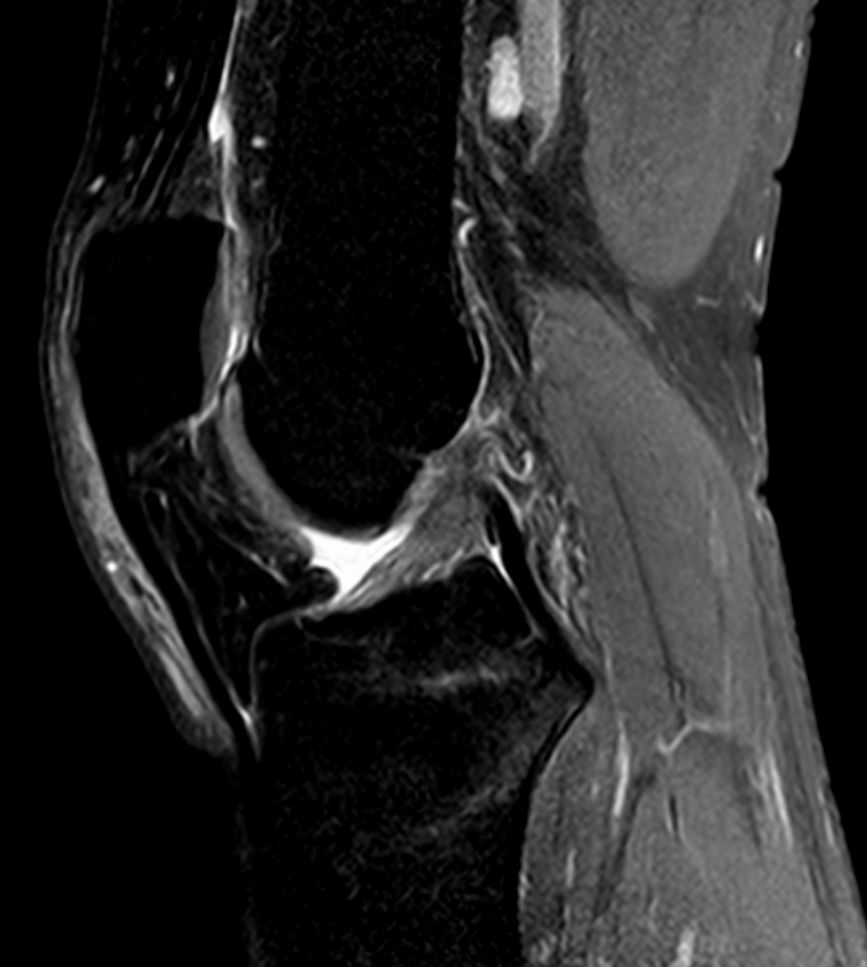
\includegraphics[height=44mm]{img/commons/acl_tear.jpg}
  \caption{ACL rupture, sagittal. A normal ACL is a dark, straight band; a ruptured one is interrupted or missing. Bright fluid fills the joint.}
\end{subfigure}\hfill
\begin{subfigure}[t]{0.33\linewidth}\centering
  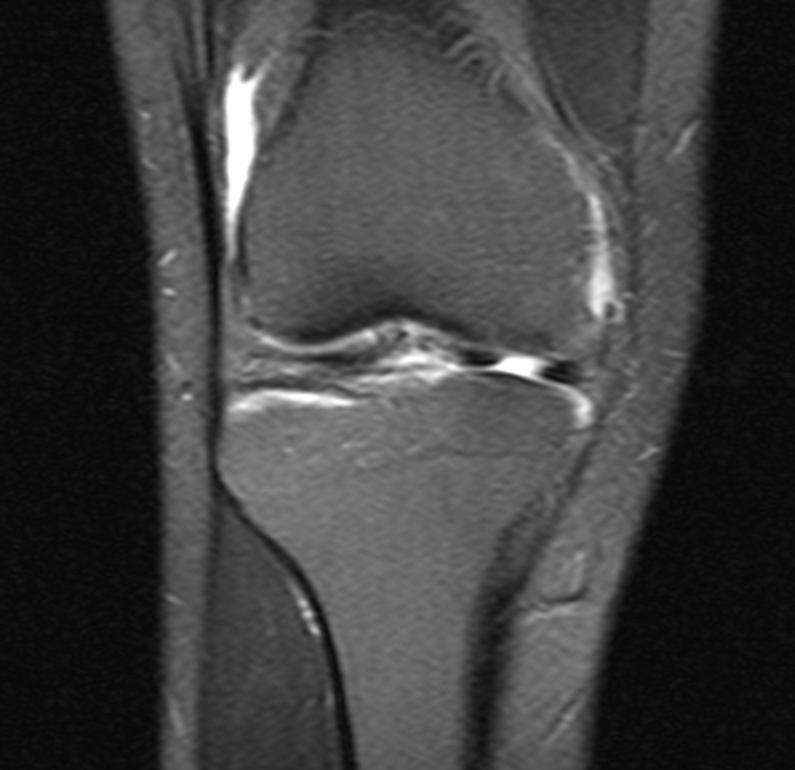
\includegraphics[height=44mm]{img/commons/meniscus_tear.jpg}
  \caption{Meniscus tear, coronal. A normal meniscus is a dark wedge; a tear shows up as a bright line inside it.}
\end{subfigure}\hfill
\begin{subfigure}[t]{0.31\linewidth}\centering
  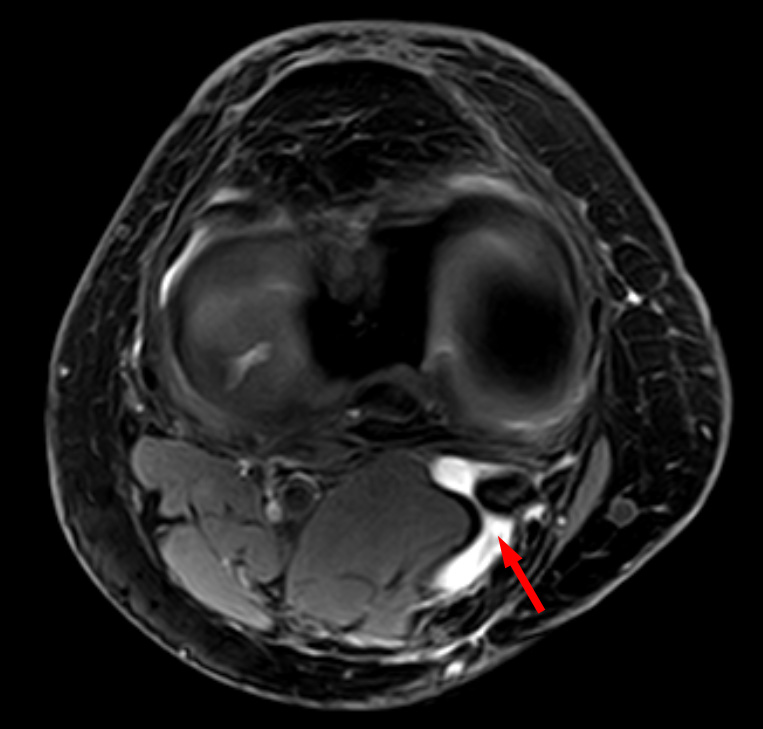
\includegraphics[height=44mm]{img/commons/baker_ax.jpg}
  \caption{Baker's cyst, axial (a slice across the leg). The arrow marks the channel between the cyst and the joint.}
\end{subfigure}
\caption{Three findings on real MRI images. All three images are fat-suppressed, so fluid is bright and fat is
dark (Chapter~\ref{ch:mri}). Images: Hellerhoff and Ciernik M, Wikimedia Commons, CC BY-SA (Appendix~\ref{app:credits}).}
\label{fig:realfindings}
\end{figure}

\begin{checkpoint}
\begin{itemize}
\done I can point to the femur, tibia, patella, both menisci, the ACL and the MCL on a drawing.
\done I know what medial, lateral and ``compartment'' mean.
\quiz Q2.1: A report says ``small joint effusion''. Is Effusion positive?
\quiz Q2.2: Which three findings share one rule about cartilage, and how do they differ?
\quiz Q2.3: Why might a model confuse Medial and Lateral Meniscus if it cannot tell a left knee from a right knee?
\end{itemize}
\end{checkpoint}
